\chapter{Fundamentación Teórica}

\label{chap:chapter1}

La base teórica funciona como el armazón conceptual sobre el cual se erige todo
trabajo investigativo. Este capítulo expone los conceptos asociados al tema, los
fundamentos teóricos existentes y el estado del arte que respaldan 
el estudio, proporcionando un sistema de referencia que orienta la comprensión 
e interpretación del fenómeno abordado. En tal sentido, 
se establece el marco conceptual necesario para contextualizar y dar sentido a 
la propuesta de solución que se desarrolla en los capítulos subsiguientes.

Además, se efectúa una comparación entre soluciones homólogas existentes para determinar características
predominantes y conocer las tendencias en este tipo de sistemas. También se 
realiza un análisis de las diferentes herramientas y tecnologías para dar a conocer
el conjunto de utensilios que serán protagonistas en el desarrollo de la propuesta de
solución, así como la metodología de desarrollo de software que guiará todo el proceso práctico.

\section{Conceptos asociados al tema}

En este epígrafe se desglosan los conceptos esenciales que convergen en el
núcleo del estudio. La clarificación de
estos términos no solo delimita el campo de acción, sino que también
proporciona el lenguaje común y la base teórica necesaria para el diseño de
una solución coherente y efectiva. Esta precisión conceptual resulta fundamental, 
pues sienta las bases sobre las cuales se articularán posteriormente las decisiones 
de diseño e implementación de la propuesta.

\subsection{Ingeniería de Líneas de Productos de Software (SPLE)}

La \ac{SPLE} es una estrategia de
ingeniería de software que busca producir familias de sistemas de software
similares a partir de un conjunto común de activos centrales mediante un
proceso gestionado de desarrollo y gestión de la variabilidad. El objetivo
principal es lograr la reutilización a gran escala, lo que se traduce en una reducción
de costos, menor tiempo de comercialización y mayor calidad de los
productos \citep{sgbuzz_lps}. El concepto de
\ac{SPL} surgió a finales de los años 90 como respuesta directa a la crisis de
productividad que enfrentaba la industria del software a pesar de las técnicas
de reutilización orientadas a objetos. La \ac{SPLE} formaliza una práctica que ya
existía intuitivamente en muchas empresas: construir un software base
(plataforma) para generar rápidamente múltiples productos similares con
variaciones controladas \citep{academialab_linea_productos}

\textbf{Conceptos Clave de SPL:}
\begin{enumerate}
    \item \textbf{Línea de Productos:} Es la familia completa de sistemas de software
    que pueden ser generados. Representa el espacio de posibilidades
    definido por el conjunto de activos.
    \item \textbf{Activos Centrales (\textit{Core Assets}):} Son los componentes fundamentales
    (código, arquitectura, modelos de diseño, documentación, planes de
    prueba) diseñados específicamente para ser compartidos y reutilizados
    en toda la línea. La inversión inicial en estos activos es clave para el
    éxito de la estrategia.
    \item \textbf{Variabilidad:} Es la propiedad esencial de una \ac{SPL}. Define la capacidad
    de la línea para ser adaptada, personalizada o configurada para generar
    productos específicos que satisfagan las necesidades particulares de un
    cliente o escenario. La variabilidad es, en esencia, el conjunto de
    diferencias controladas entre los productos posibles.
    \item \textbf{Puntos de Variabilidad (\textit{Variability Points}):} Son las ubicaciones
    explícitas dentro de los Activos Centrales donde se deben tomar
    decisiones para configurar un producto. Estos puntos actúan como
    "interruptores" o "opciones" que guían el proceso de personalización.
\end{enumerate}

La motivación detrás de la \ac{SPL} es fundamentalmente económica y técnica,
pues permite el ahorro de costos, ya que al compartir la gran mayoría de los
activos (entre el 70\% y 90\% del sistema), se evita la reimplementación del
mismo código y diseño para cada nuevo producto, además, provee de una reducción del tiempo de comercialización (\textit{Time-to-Market}) pues la creación de
un nuevo producto se reduce de un ciclo completo de desarrollo a un simple
proceso de configuración y ensamblaje de activos preexistentes y permite una
mejora de la calidad, pues como los activos centrales, al ser reutilizados y
probados en múltiples productos, alcanzan un nivel de madurez y robustez
superior al que podría lograrse en un desarrollo de producto único \citep{ingenieria_software_lps}.

La \ac{SPL} opera a través de dos procesos interdependientes que deben
gestionarse de manera continua, siendo el primero de estos la Ingeniería del
Dominio (\textit{Domain Engineering}), proceso hacia arriba que se enfoca en la
creación y el mantenimiento de los Activos Centrales, cuya tarea principal es el
modelado de la variabilidad para comprender y documentar todas las posibles
configuraciones que la línea puede soportar y que constituye la base teórica y
formal de la línea, y un segundo, la Ingeniería de la Aplicación (\textit{Application
Engineering}), el cual es el proceso hacia abajo que utiliza los Activos Centrales
para configurar y generar productos específicos, que implica tomar las
decisiones de variabilidad definidas en el modelo (seleccionar las opciones)
para producir una instancia concreta de la línea de productos. La herramienta
principal y estándar de facto para formalizar y gestionar la variabilidad durante
la Ingeniería del Dominio es el \ac{FM}.
Este modelo establece el puente formal entre las opciones de la línea de
productos y la capacidad de generar una instancia válida, lo cual es el principio
que se busca trasladar al diseño curricular.

La búsqueda de la variabilidad curricular ha llevado a la exploración 
de paradigmas de ingeniería de software. El concepto de \ac{SPL}
ofrece un enfoque estructurado y probado para gestionar familias de productos
a partir de un conjunto común de activos \citep{apel2013feature}. Cuando este
paradigma se aplica al dominio educativo, surge el concepto de "Líneas de
Productos Educativos", donde un tronco curricular común puede derivar en
múltiples planes de estudio especializados mediante la gestión explícita de su
variabilidad.

\subsection{Ingeniería de Líneas de Productos de Software (SPLE)}

Es necesario contar con un modelo que represente de manera explícita las
variaciones y opciones disponibles en la línea de productos. Este modelo
debe ser capaz de capturar la complejidad de las relaciones entre las
características y sus variaciones, así como las restricciones que pueden
existir entre ellas \citep{pohl2005software}. La representación gráfica de 
estas relaciones es fundamental para facilitar la comprensión y el análisis 
de la variabilidad en la línea de productos.

El Modelo de Características (\textit{Feature Model} - \ac{FM}) es la técnica de modelado
central en la Ingeniería de Líneas de Productos de Software. Su formalismo es
indispensable para pasar de la noción abstracta de variabilidad a una
representación estructurada y analizable \citep{ptc_feature_models}. 
Los Modelos de Características fueron formalmente introducidos por \citet{kang1990foda} 
como parte de la metodología \ac{FODA}, un enfoque pionero para la ingeniería de dominios. 
Desde su concepción, un \ac{FM} ha sido reconocido como el artefacto
primario para la captura de la variabilidad funcional de un sistema. En esencia,
un \ac{FM} es un modelo de dominio que no solo documenta las posibles
funcionalidades, sino que también define las reglas de composición entre ellas
\citep{gfg_feature_engineering}.
            
Formalmente, un Modelo de Características se define como un árbol de
decisiones jerárquico donde cada nodo es una característica (\textit{feature}). Una
característica se entiende como una unidad de funcionalidad, un requisito, o un
aspecto distintivo de un sistema, tal como es percibido por el usuario final o el
analista del dominio.

La estructura del \ac{FM} es un árbol de composición, donde:
\begin{itemize}
    \item La Característica Raíz representa el sistema o la línea de producto
    completa (ej., la carrera de Ingeniería Informática).
    \item Las características descendientes detallan la composición de sus
    características padre hasta alcanzar las características hoja, que son las
    unidades más pequeñas y configurables.
\end{itemize}

\textbf{Relaciones estructurales}
La potencia del \ac{FM} reside en su notación gráfica concisa, la cual utiliza la
posición y símbolos específicos para codificar las restricciones de
configuración. Las relaciones entre una característica padre (letra P) y sus hijos (letra C) definen
las decisiones de inclusión o exclusión; véase la Tabla~\ref{tab:relaciones_estructurales_FM} 
\citep{pohl2005software, kang1990foda, benavides2010PrinciplesFM, benavides2010automated, wang2007FormalSemanticsFM}.
                        
\begin{longtable}{|p{5cm}|p{5cm}|p{5cm}|}
    \caption{Notación semántica de las relaciones entre características de los \ac{FM} \label{tab:relaciones_estructurales_FM}}\\
    \hline
    \rowcolor[HTML]{CBCEFB} 
    \textbf{Relación} & \textbf{Semántica Formal} & \textbf{Implicación en la Configuración} \\
    \hline
    \endfirsthead
                
    \multicolumn{3}{c}
	{{\bfseries \tablename\ \thetable{} -- Continuación de la página anterior}} \\
                
    \hline
    \rowcolor[HTML]{CBCEFB} 
    \textbf{Relación} & \textbf{Semántica Formal} & \textbf{Implicación en la Configuración} \\
    \hline
    \endhead
                
    \hline
    \multicolumn{3}{|r|}{{Continúa en la siguiente página}} \\
    \endfoot
                
    \hline
    \endlastfoot
                
    % Cuerpo de la tabla
    Obligatoa lipa tinyria & $P \rightarrow C$ & Si el padre P es seleccionado, el hijo obligatorio C debe incluirse. No hay variabilidad en este punto \\ 
    \hline
    \rowcolor[HTML]{EDEBF1}
    Opcional & $C \rightarrow P $ & El hijo C puede ser incluido o excluido, si se selecciona el padre P. Introduce variabilidad \\ 
    \hline
    Agrupación AND & $\left(P \rightarrow \bigwedge_{i=1}^{n} C_i\right) \land \bigwedge_{i=1}^{n} (C_i \rightarrow P)$ & Si se selecciona la característica padre P, todos los hijos Ci deben incluirse; cada hijo seleccionado implica la presencia del padre. No introduce variabilidad dentro del grupo \\
    \hline
    \rowcolor[HTML]{EDEBF1}
    Agrupación OR & $\left(P \rightarrow \bigvee_{i=1}^{n} C_i\right) \land \bigwedge_{i=1}^{n} (C_i \rightarrow P)$ & Al seleccionar el padre P, debe elegirse al menos un hijo Ci. Cada hijo seleccionado requiere que el padre esté presente. Sí introduce variabilidad \\
    \hline
    Agrupación alternativa & $\left(P \rightarrow \bigvee_{i=1}^{n} C_i\right) \land \bigwedge_{i \neq j} \neg(C_i \land C_j) \land \bigwedge_{i=1}^{n} (C_i \rightarrow P)$ & Cuando el padre P se selecciona, exactamente un hijo Ci puede activarse y la elección de cualquier hijo obliga a seleccionar al padre. Sí introduce variabilidad \\
    \hline
\end{longtable}

La figura \ref{fig:relaciones_estructurales_FM} muestra los símbolos gráficos para representar las relaciones estructurales.
\begin{figure}[H]
    \centering
    \captionbox{Símbolos gráficos para representar las relaciones estructurales. \label{fig:relaciones_estructurales_FM}}
    {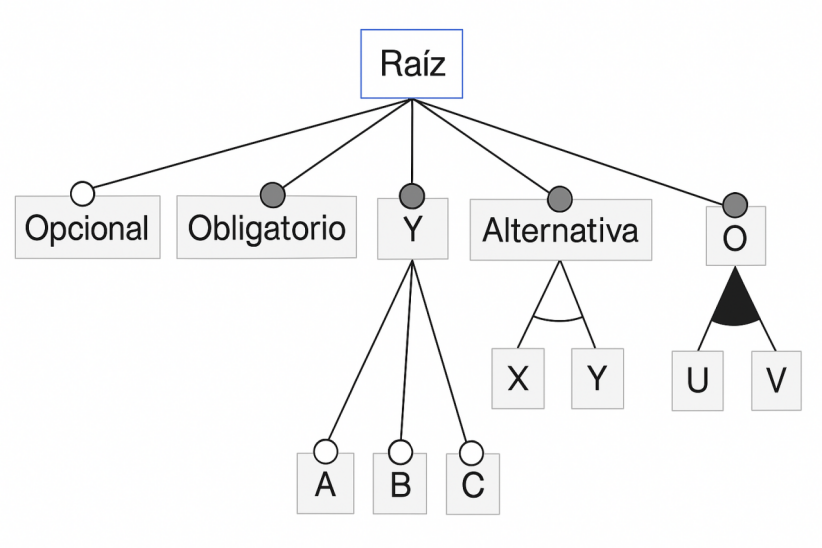
\includegraphics[width=1\linewidth]{Images/feature_models.png}}
\end{figure}

\textbf{Restricciones (\textit{Cross-Tree})}

Las relaciones jerárquicas son insuficientes para capturar todas las reglas de
negocio complejas. Por ello, los \ac{FM} permiten definir las restricciones transversales 
(\textit{cross-tree}); que son reglas lógicas que definen
dependencias entre características que no están directamente conectadas en
la jerarquía padre-hijo del árbol de características. Su función es garantizar la
validez de una configuración al capturar las relaciones complejas del mundo
real que la estructura jerárquica por sí sola no puede expresar 
\citep{sundermann2023sat,benavides2005Taxonomy}.

Las dos formas más comunes y fundamentales son:
\begin{itemize}
    \item \textbf{Requiere:} Esta restricción establece una dependencia de presencia. Si
    una característica A requiere una característica B, entonces siempre que
    A sea seleccionada en una configuración, B también debe estarlo. Porejemplo, en un modelo de características para un automóvil, la
    característica "Navegación" puede requerir la característica "Pantalla
    Táctil". Esta relación se modela en lógica proposicional como el
    condicional $A \rightarrow B$ \citep{sundermann2023sat, benavides2005Taxonomy}.
    \item \textbf{Excluye:} Esta restricción establece un conflicto o incompatibilidad. Si
    una característica C excluye una característica D, entonces ambas no
    pueden formar parte de la misma configuración. Por ejemplo, el motor
    "Diésel" puede excluir la transmisión "Eléctrica" en un vehículo híbrido.
    Su representación lógica es la negación de la conjunción: $\neg(C \land D)$
    \citep{sundermann2023sat, benavides2005Taxonomy}.
\end{itemize}

\textbf{Semántica Formal y Solucionadores SAT (\textit{SAT Solvers})}

La semántica formal de un \ac{FM} proporciona un
significado matemático preciso a todos sus elementos (jerarquía, relaciones y
restricciones), lo que permite un análisis automático y libre de ambigüedades.
\begin{itemize}
    \item \textbf{Traducción a Lógica Proposicional:} La base de la semántica formal es
    la traducción de todo el \ac{FM} a una fórmula en lógica proposicional. Cada
    característica se representa como una variable proposicional (que puede
    ser Verdadera o Falsa, indicando si está seleccionada o no). Las
    relaciones padre-hijo y las restricciones cross-tree se convierten en una
    serie de fórmulas lógicas que, en conjunto, definen el conjunto de todas
    las configuraciones válidas \citep{sundermann2023sat, thum2014featureide}.
    \item \textbf{Satisfacibilidad (\ac{SAT}) y \ac{SHARPSAT}:} Una vez el \ac{FM} está representado como
    una fórmula lógica F, se pueden realizar diversos análisis:
        \begin{itemize}
            \item \textbf{Análisis de \ac{SAT}:} Consiste en verificar si existe al menos una
            asignación de valores (Verdadero/Falso) a las variables que haga
            que la fórmula F sea verdadera. Esto responde a la pregunta
            fundamental de si el \ac{FM} tiene al menos una configuración válida
            \citep{sundermann2023sat, benavides2010automated,mendonca2009SAT}.
            \item \textbf{Análisis de \ac{SHARPSAT}:} Consiste en el conteo de modelos (\textit{Model Counting}) que
            satisfacen F. Esto es crucial para determinar el número total de configuraciones válidas que
            define un \ac{FM}, una métrica esencial para comprender su
            variabilidad y complejidad \citep{sundermann2023sat, benavides2010automated,mendonca2009SAT}.
        \end{itemize}
    \item \textbf{Solucionadores SAT (\textit{SAT solvers}):} Un solucionador SAT (\textit{SAT solver}) es una herramienta algorítmica altamente
    optimizada diseñada para resolver problemas de satisfacibilidad. Dada
    una fórmula F, el solucionador (\textit{solver}) determina si es satisfacible (\ac{SAT}) o insatisfacible
    (UNSAT). Para el análisis de \ac{SHARPSAT}, se emplean solucionadores especializados de conteo de modelos (\textit{\#SAT solvers})
    como sharpSAT y Ganak, que han demostrado un
    rendimiento excelente al calcular el número de configuraciones en
    modelos industriales \citep{sundermann2023sat, soos2020Ganak}.
\end{itemize}






















\begin{figure}[!htb]
\centering
\captionbox{Vista del Arco de Moncloa\label{fig:DSC00461}}
{
\includegraphics[width=0.7\linewidth]{Images/DSC00461}}
\end{figure}

En la Tabla \ref{Prueba} se observa \dots\\

\begin{table}[!h]
\centering
\captionbox{Caption de Prueba\label{Prueba}}
{
	\begin{tabular}{lllll}
	\hline \textbf{No. 1} & \textbf{No. 2} & \textbf{No. 3} & \textbf{No. 4} & \textbf{No. 5}\\ \hline
	12 & 12 & 56 & 56 &  56 \\ 
	12 & 12 & 56 & 56 &  56 \\
	\hline 
	\end{tabular}
}
\end{table}


